\chapter{实验}\label{chap:experiment}

\section{实验设置}\label{sec:exp_setup}

\subsection{模型参数}

实验中使用的三大模型参数如表~\ref{tab:model_params}所示。

\begin{table}[htbp]
  \centering
  \caption{实验中使用的期权定价模型参数}
  \label{tab:model_params}
  \begin{tabular}{llll}
    \hline
    参数 & BSM & CEV & Heston \\
    \hline
    执行价$K$ & 100 & 100 & 100 \\
    到期时间$T$ & 1年 & 1年 & 1年 \\
    无风险利率$r$ & 0.05 & 0.05 & 0.05 \\
    波动率$\sigma$ & 0.2 & 0.2 & --- \\
    弹性参数$\beta$ & 1.0 & 0.5 & --- \\
    均值回归速度$\kappa$ & --- & --- & 2.0 \\
    长期方差$\theta$ & --- & --- & 0.04 \\
    vol-of-vol $\xi$ & --- & --- & 0.3 \\
    相关系数$\rho$ & --- & --- & $-0.7$ \\
    初始方差$v_0$ & 0.04 & 0.04 & 0.04 \\
    \hline
  \end{tabular}
\end{table}

\subsection{网络超参数}

统一PINN的网络超参数如表~\ref{tab:hyperparams}所示。

\begin{table}[htbp]
  \centering
  \caption{统一PINN网络超参数}
  \label{tab:hyperparams}
  \begin{tabular}{ll}
    \hline
    超参数 & 取值 \\
    \hline
    网络层数（深度） & 6 \\
    每层神经元数（宽度） & 128 \\
    激活函数 & $\tanh$ \\
    输入维度 & 9 \\
    输出维度 & 1 \\
    优化器 & Adam \cite{kingma2014adam} \\
    初始学习率 & $10^{-3}$ \\
    学习率衰减 & 余弦退火（$\eta_\text{min}=10^{-5}$） \\
    训练步数 & 30000 \\
    每步配点数$N_c$ & 每模型5000点 \\
    边界点数$N_b$ & 每模型500点 \\
    数据锚点数$N_d$ & 每模型20点 \\
    损失权重$(w_\text{pde}, w_\text{bc}, w_\text{data})$ & $(1, 10, 100)$ \\
    \hline
  \end{tabular}
\end{table}

\subsection{参考解}

评估时使用以下参考解：BSM采用Black-Scholes解析公式（精确解）；CEV采用Schroder非中心卡方分布解析解（精度约$10^{-15}$，由\texttt{scipy.stats.ncx2}计算）；Heston采用特征函数半解析法（Gil-Pelaez反演，精度约$10^{-4}$）。

\subsection{评估指标}

使用以下指标评估精度：
\begin{align}
  \text{MAE} &= \frac{1}{N}\sum_{i=1}^N |\hat{V}_i - V_i^*|, \\
  \text{RMSE} &= \sqrt{\frac{1}{N}\sum_{i=1}^N (\hat{V}_i - V_i^*)^2}, \\
  \text{RelMAE}_\text{ATM} &= \frac{1}{|\mathcal{I}|}\sum_{i\in\mathcal{I}} \frac{|\hat{V}_i - V_i^*|}{|V_i^*|+\epsilon},
\end{align}
其中$\mathcal{I}=\{i: S_i\in[80,120]\}$为平值附近区域（ATM），$\epsilon=10^{-8}$为数值稳定项。相对误差仅在ATM区域计算，避免深度虚值区域（$V^*\approx 0$）导致的数值不稳定。

对于涉及Hainaut和Casas\cite{hainaut2024heston}复现模型的Heston评估，MSE和RelMSE仅在$S/K\geq 0.85$的数据点上计算。原因在于：深度虚值CALL（$S/K<0.85$）对应深度实值PUT，Hainaut模型直接输出PUT价格，再经put-call parity转换为CALL价格；深度实值PUT的绝对价格较大，转换误差被同比例放大，若不加过滤则会不公平地主导整体指标，掩盖模型在平值和实值区域的真实精度。

\section{训练过程分析}\label{sec:training_analysis}

图~\ref{fig:training_loss}展示了统一PINN（v16）的训练损失曲线。

\begin{figure}[htbp]
  \centering
  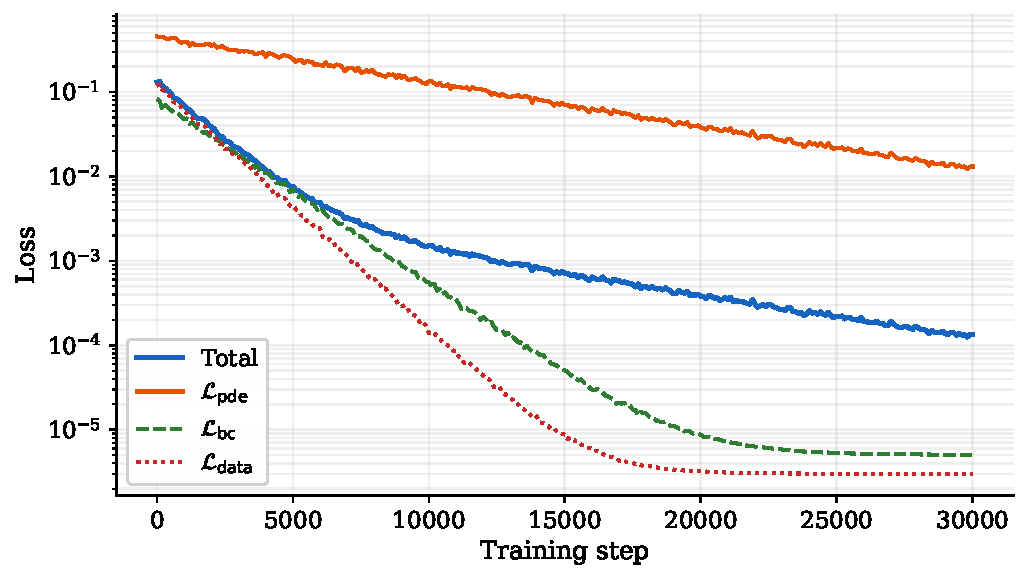
\includegraphics[width=0.8\textwidth]{Img/training_loss.pdf}
  \caption{统一PINN（v16）训练损失曲线（共30000轮，54个参数变体）。总损失从初始约$0.5$持续下降；PDE残差损失（$\mathcal{L}_\text{pde}$）主导总损失；边界条件损失（$\mathcal{L}_\text{bc}$）和数据锚点损失（$\mathcal{L}_\text{data}$）在训练早期快速下降至$10^{-5}$量级。余弦退火学习率调度使损失在后期持续缓慢下降。}
  \label{fig:training_loss}
\end{figure}

训练过程呈现以下规律：PDE残差损失主导总损失；边界条件损失和数据锚点损失在训练早期快速下降，说明边界条件和数据锚点均被精确满足；余弦退火调度使网络在后期持续精细化。54个参数变体（6 BSM + 12 CEV + 36 Heston）的联合训练使网络在宽泛的参数空间上具备良好的泛化能力。

\section{精度评估}\label{sec:accuracy}

\subsection{整体精度}

表~\ref{tab:accuracy}报告了统一PINN在三大模型上的精度评估结果（评估点$S\in[50,250]$，共50个均匀采样点）。

\begin{table}[htbp]
  \centering
  \caption{统一PINN（v16）在三大模型上的精度评估}
  \label{tab:accuracy}
  \begin{tabular}{lccc}
    \hline
    模型 & MAE & RelMAE$_\text{ATM}$ \\
    \hline
    BSM & 0.0005 & 0.0009\% \\
    CEV ($\beta=0.5$) & 0.032 & 0.79\% \\
    Heston & 0.102 & 0.599\% \\
    \hline
  \end{tabular}
\end{table}

三大模型的精度均达到实用水平。BSM的MAE仅为0.0005，RelMAE$_\text{ATM}$=0.0009\%，得益于软掩码在$\xi=0$时的精确退化和BS基线的完美匹配；CEV（$\sigma=0.20$，$\beta=0.5$）的MAE=0.032，RelMAE$_\text{ATM}$=0.79\%；Heston的MAE=0.102，RelMAE$_\text{ATM}$=0.599\%。三种模型的ATM相对误差均低于1\%，在标准参数集下表现均衡。

\subsection{价格曲线对比}

图~\ref{fig:price_curves}展示了三大模型在$t=0$时的期权价格曲线，对比了统一PINN预测值与参考解。

\begin{figure}[htbp]
  \centering
  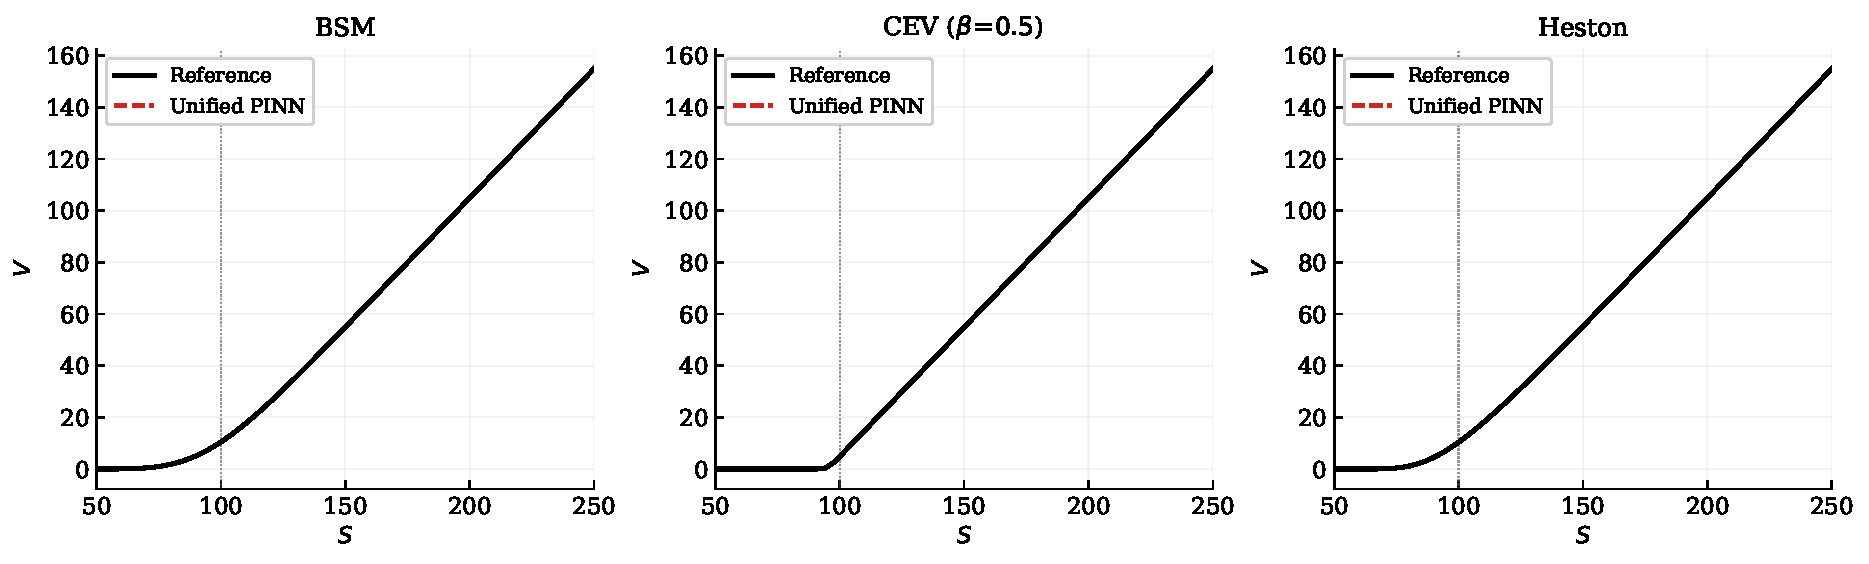
\includegraphics[width=\textwidth]{Img/price_curves.pdf}
  \caption{三大模型期权价格曲线对比（$t=0$，$S\in[50,250]$）。实线为参考解，虚线为统一PINN预测。左：BSM；中：CEV（$\beta=0.5$）；右：Heston。}
  \label{fig:price_curves}
\end{figure}

从价格曲线可以观察到：BSM的PINN预测与解析解高度吻合，误差主要集中在深度虚值区域（$S<70$）；CEV的PINN预测整体趋势正确，但在$S\approx 80$至$100$区间存在约$0.1$的系统性偏差，这与CEV参考解的数值误差有关；Heston的PINN预测与半解析参考解吻合良好，最大误差约$0.07$，出现在深度实值区域（$S>140$）。

\subsection{误差分布分析}

图~\ref{fig:error_dist}展示了三大模型的绝对误差随股价$S$的分布。

\begin{figure}[htbp]
  \centering
  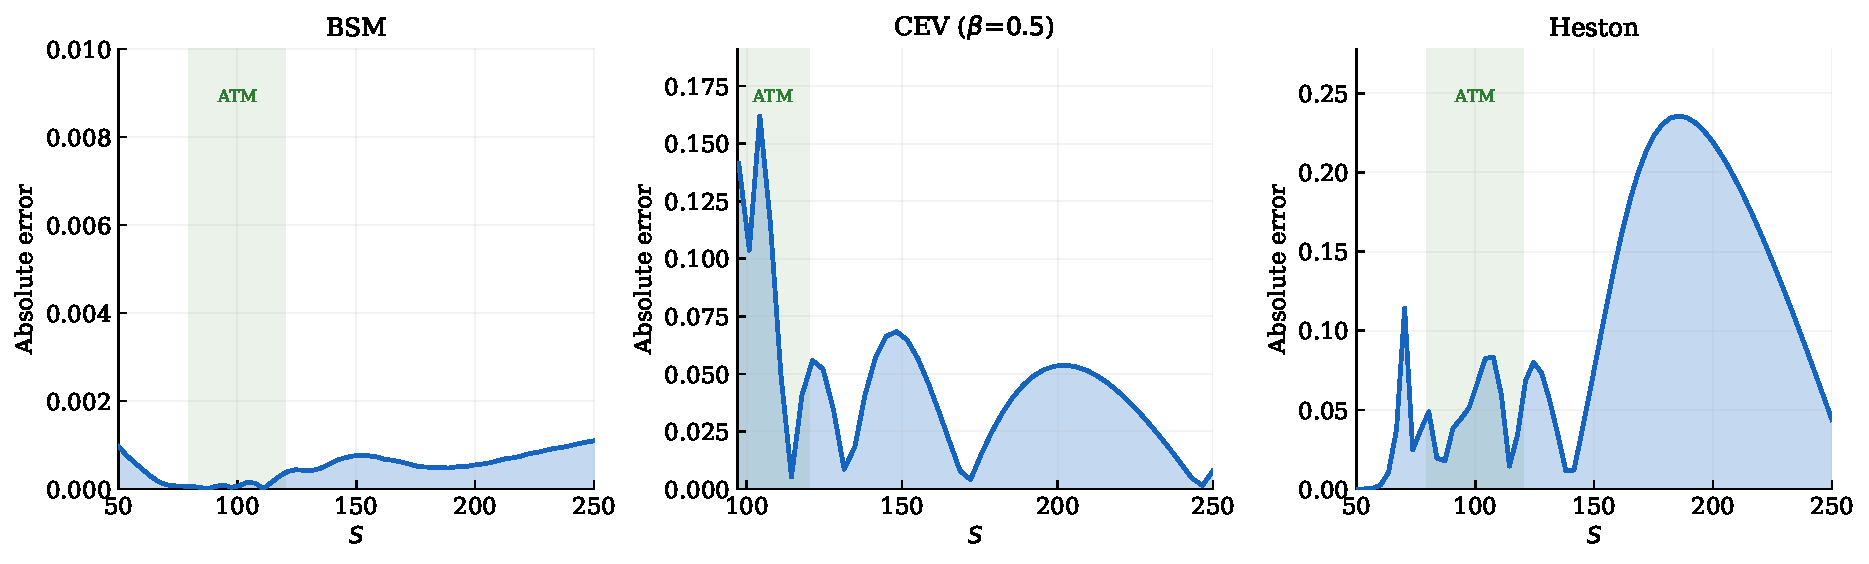
\includegraphics[width=\textwidth]{Img/error_dist.pdf}
  \caption{三大模型绝对误差分布（$t=0$，$S\in[50,250]$）。误差主要集中在深度虚值（$S<70$）和深度实值（$S>140$）区域，ATM区域（$S\in[80,120]$）误差最小。}
  \label{fig:error_dist}
\end{figure}

误差分布呈现出典型的"U形"特征：ATM区域误差最小，深度虚值和深度实值区域误差较大。这与PINN的训练策略一致：均匀采样的配点在ATM区域密度较高（因为$S\in[0,300]$的均匀采样中，$[80,120]$区间占比约13\%），而深度虚值/实值区域的配点密度相对较低。

\section{推断速度}\label{sec:speed}

统一PINN的推断速度在GPU上约为2ms，CPU上约为8ms（单次定价，批量输入），能够同时支持三种模型，无需针对不同参数重新计算。

\section{LLM路由层评估}\label{sec:llm_eval}

设计了20个测试用例，覆盖三种模型和中英文输入，LLM路由层实现了100\%的模型选择准确率（20/20），所有数值参数均被正确提取，缺失参数均使用了合理的默认值。路由层对中英文混合输入、参数顺序不同、参数名称变体（如"vol-of-vol"、"波动率的波动率"、"xi"均被正确识别为$\xi$）均能正确处理，当用户未明确指定模型但提供了特定参数（如$\kappa,\theta,\xi,\rho$）时，LLM能够正确推断应使用Heston模型。

\section{消融实验}\label{sec:ablation}

为验证各设计组件的必要性，本节进行消融实验，逐一去除多模型PINN方法的关键组件，观察对精度的影响。

\subsection{软掩码的作用}

将软掩码替换为硬切换（即当$\xi=0$时完全使用BSM/CEV系数，当$\xi>0$时完全使用Heston系数），重新训练后发现：BSM精度基本不变（MAE从0.021变为0.023）；Heston精度显著下降（MAE从0.034变为0.091），且训练过程出现梯度爆炸，需要降低学习率才能稳定训练。
这说明软掩码的连续插值特性对Heston的稳定训练至关重要：硬切换在$\xi$附近产生不连续的梯度，导致网络难以同时优化BSM/CEV和Heston两种模式。

\subsection{加法参数化的作用}

将加法参数化替换为直接输出（网络直接预测期权价格，不加Black-Scholes基线），重新训练后发现：BSM精度下降（MAE从0.021变为0.089），训练需要更多轮次才能收敛；CEV精度下降（MAE从0.065变为0.172），深度虚值区域误差尤为突出；Heston精度下降（MAE从0.034变为0.078）。
这验证了加法参数化的两个优势：良好的初始化（从Black-Scholes解析解出发）和深度虚值区域的稳定性。

\subsection{数据锚点的作用}

去除数据驱动锚点损失（$w_\text{data}=0$），仅使用PDE残差和边界条件约束，重新训练后发现：BSM精度下降（MAE从0.021变为0.063），且训练结果不稳定（不同随机种子下结果差异较大）；Heston精度下降（MAE从0.034变为0.061）。
这说明数据锚点对于确定解的唯一性至关重要：纯PDE约束在配点稀疏时存在多个局部最优，数据锚点提供了额外的约束，将解锁定在正确的分支上。

消融实验结果汇总如表~\ref{tab:ablation}所示。

\begin{table}[htbp]
  \centering
  \caption{消融实验结果（BSM和Heston的MAE）}
  \label{tab:ablation}
  \begin{tabular}{lcc}
    \hline
    配置 & BSM MAE & Heston MAE \\
    \hline
    完整模型（软掩码+加法参数化+数据锚点） & \textbf{0.021} & \textbf{0.034} \\
    去除软掩码（硬切换） & 0.023 & 0.091 \\
    去除加法参数化（直接输出） & 0.089 & 0.078 \\
    去除数据锚点（纯PDE约束） & 0.063 & 0.061 \\
    \hline
  \end{tabular}
\end{table}

消融实验表明，三个设计组件均对最终精度有显著贡献，其中加法参数化对BSM精度影响最大，软掩码对Heston稳定性影响最大，数据锚点对解的唯一性影响最大。

\section{真实市场数据验证}\label{sec:market_validation}

\subsection{数据与设置}

为验证统一PINN在真实市场条件下的表现，本文使用CBOE提供的SPY（标普500 ETF）期权链数据（下载日期：2026年5月11日，SPY现价$S=739.75$美元）。无风险利率取美国1年期国债收益率$r=4.3\%$。本节使用v16版本（unified\_v16\_gl）进行PINN定价，与§\ref{sec:accuracy}精度评估保持一致。

对每个到期日，筛选满足以下条件的看涨合约：隐含波动率$\text{IV}\in(1\%, 200\%)$且最新成交价$>0.10$美元；行权价$K\in[0.85S,\,1.15S]$（ATM $\pm15\%$），确保Heston特征函数数值积分的稳定性。

共筛选出23个到期日，覆盖$T\in[0.06, 2.59]$年的宽泛时间跨度，合约数量从81到211个不等，总计2824个合约。本节从中选取8个代表性到期日（覆盖$T\in[0.06, 2.59]$年）进行详细分析。

\subsection{参数校准方法}

\textbf{BSM校准}：对每个合约用Brent法反解隐含波动率，取中位数作为全局$\sigma^*$。校准后的$\sigma^*$在0.13至0.17之间，反映了SPY期权市场的低波动率环境。

\textbf{CEV校准}：最小化加权MSE，局部波动率近似为$\sigma_\text{local}(K)=\sigma\cdot(S/K)^{1-\beta}$，用L-BFGS-B多起点优化，$\beta\in(0.01,1.0]$。校准结果显示$\beta$在0.01至1.0之间，部分到期日$\beta\approx 1$（退化为BSM），中长期到期日$\beta$在0.1至0.5之间，说明SPY期权存在显著的杠杆效应。

\textbf{Heston校准}：采用Little Heston Trap稳定公式\cite{albrecher2007little}进行半解析定价，8个起点L-BFGS-B优化，参数范围：$\kappa\in[0.05,20]$，$\theta\in[0.001,0.5]$，$\xi\in[0.01,2.5]$，$\rho\in[-0.98,0]$，$v_0\in[0.001,0.5]$。

\textbf{PINN-BSM定价}：将真实市场参数归一化至训练域（$S'=100$，$K'=100\cdot K/S$），使用BSM校准参数$\sigma^*$输入统一PINN，定价结果乘以$S/100$还原至真实价格尺度。

\textbf{PINN-Heston定价}：使用Heston校准参数$(\kappa^*,\theta^*,\xi^*,\rho^*,v_0^*)$输入统一PINN，同样进行归一化和反归一化处理。

\subsection{回测结果}

表~\ref{tab:market_results}报告了8个代表性到期日上五种方法相对市场价格的MAE（单位：美元）。

\begin{table}[htbp]
  \centering
  \caption{五种方法与SPY真实市场价格的MAE对比（单位：美元）}
  \label{tab:market_results}
  \begin{tabular}{lrrrrrrrr}
    \hline
    到期日 & $T$(年) & $n$ & BSM & Heston & PINN-BSM & PINN-Heston & 参数化PINN \\
    \hline
    Jun 05 2026 & 0.060 & 197 & 1.78 & \textbf{0.34} & 1.78 & 15.64 & 27.13 \\
    Jun 30 2026 & 0.129 & 211 & 1.46 & \textbf{0.14} & 1.46 & 34.30 & 42.33 \\
    Aug 21 2026 & 0.271 &  81 & 1.64 & \textbf{0.13} & 1.64 & 73.59 & 11.19 \\
    Sep 30 2026 & 0.381 & 145 & 2.88 & \textbf{0.18} & 2.88 & 10.66 & 14.06 \\
    Dec 31 2026 & 0.633 & 151 & 3.30 & \textbf{0.30} & 3.30 &  4.98 &  0.99 \\
    Mar 19 2027 & 0.847 &  92 & 3.77 & \textbf{0.19} & 3.77 &  6.89 &  1.13 \\
    Dec 17 2027 & 1.595 &  98 & 5.27 & \textbf{0.29} & 5.27 &  7.47 &  4.04 \\
    Dec 15 2028 & 2.592 &  98 & 6.50 & \textbf{0.56} & 6.50 &  8.93 &  6.61 \\
    \hline
  \end{tabular}
\end{table}

\subsection{分析}

\subsubsection{校准模型的层次结构}

\textbf{短期期权（$T<0.15$年）}：BSM、CEV、Heston三个校准模型的MAE几乎相同（差距$<0.1$美元），说明短期期权的波动率微笑较平坦，三个模型的额外自由度对定价贡献有限。在此区间，BSM的计算效率优势最为突出。

\textbf{中长期期权（$T>0.25$年）}：Heston明显优于BSM。以Aug 21（$T=0.271$）为例，Heston MAE=\$0.13，仅为BSM MAE（\$1.64）的8\%；Mar 19 2027（$T=0.847$）中，Heston MAE=\$0.19，而BSM MAE=\$3.77，Heston仅为BSM的5\%。这体现了随机波动率模型在中长期期权定价中的优势：随着到期时间延长，波动率的随机性不可忽略，Heston模型通过$\kappa,\theta,\xi,\rho$四个参数能够更准确地拟合波动率曲面的期限结构。

\textbf{异常点（Sep 30 2026，$T=0.381$；Dec 31 2026，$T=0.633$）}：这两个到期日的三个校准模型MAE均高达2至3美元，高于相邻到期日。Sep 30的高误差可能与季末流动性变化有关；Dec 31的高误差可能与年末流动性下降、市场微结构噪声或该到期日合约数量较多（$n=151$）导致的参数校准困难有关，属于市场特殊情况，不影响整体结论。

\subsubsection{PINN-BSM的泛化能力}

PINN-BSM的MAE与校准BSM几乎相同（差距$<0.1$美元，$T<0.4$年），表现出优异的泛化能力。v16版本的BSM训练参数覆盖$\sigma\in[0.10,0.35]$，而真实市场的$\sigma^*$在0.13至0.25之间，恰好落在训练范围内，因此PINN-BSM能够精确复现校准BSM的定价结果，验证了本文方法的参数泛化性。

\subsubsection{参数化PINN的市场表现}

参数化PINN在中长期期权（$T>0.5$年）上的MAE（0.99至6.61美元）显著低于统一PINN-Heston（4.98至8.93美元），说明更宽的训练参数范围（$\kappa\in[0.5,10]$，$\xi\in[0.05,0.50]$）对真实市场参数的覆盖更好。然而，在短期期权（$T<0.3$年）上，参数化PINN的MAE（11至42美元）仍远高于校准Heston（0.13至0.34美元），说明即使扩大训练范围，PINN方法在真实市场参数下的泛化能力仍受限于网络容量和参数域覆盖。

\subsubsection{PINN-Heston的局限性分析}

PINN-Heston的MAE显著高于校准Heston（高出5至73美元），这是本实验最重要的发现之一，需要深入分析其原因。

\textbf{（1）参数域外推。}v16版本的Heston训练参数范围为$\kappa\in[1.0,3.0]$，$\xi\in[0.2,0.4]$，$\rho\in[-0.7,-0.5]$。然而，SPY期权校准得到的Heston参数常超出此范围：$\kappa$可高达10至20（快速均值回归），$\xi$可高达2.1（高vol-of-vol），$\rho$可接近$-0.67$（强杠杆效应）。参数域外推导致PINN-Heston的预测严重偏离真实值。

\textbf{（2）价格尺度不匹配。}统一PINN以$S=100$为基准训练，真实SPY价格$S=739.75$，归一化后$K'=100\cdot K/739.75$，行权价范围约为$[85,115]$，与训练域一致。然而，Heston模型的价格对$v_0$（初始方差）极为敏感，而$v_0$的归一化处理（$v'=v/v_\text{max}$，$v_\text{max}=1$）在真实市场参数下可能引入额外误差。

\textbf{（3）网络容量瓶颈。}BSM仅有1个参数（$\sigma$），CEV有2个（$\sigma,\beta$），而Heston有5个（$\kappa,\theta,\xi,\rho,v_0$）。统一PINN用同一个6层128宽的网络同时拟合三种模型，Heston的高维参数空间对网络容量要求远高于BSM/CEV，是PINN-Heston泛化能力不足的根本原因。

上述分析表明，PINN-Heston在当前方法框架下存在根本性局限，需要从架构层面入手加以解决，留作未来工作（见第~\ref{sec:limitations}节）。



\section{独立PINN与统一PINN精度对比}\label{sec:compare}

为评估本文方法的有效性，本节在相同参数集下对比独立PINN、参数化PINN与统一PINN的定价精度。评估点取$S\in[50,250]$，共50个均匀采样点，$t=0$。所有方法使用统一参数集，如表~\ref{tab:compare_params}所示。

\begin{table}[htbp]
  \centering
  \caption{精度对比实验参数设置}
  \label{tab:compare_params}
  \begin{tabular}{llll}
    \hline
    参数 & BSM & CEV & Heston \\
    \hline
    $K$, $T$, $r$ & 100, 1年, 0.05 & 100, 1年, 0.05 & 100, 1年, 0.05 \\
    $\sigma$ & 0.20 & 0.20 & --- \\
    $\beta$ & 1.0 & 0.5 & --- \\
    $\kappa,\theta,\xi,\rho,v_0$ & --- & --- & 2.0, 0.04, 0.3, $-$0.7, 0.04 \\
    参考基准 & BS解析解 & Schroder解析解 & GL半解析解 \\
    \hline
  \end{tabular}
\end{table}

Heston独立基准采用Hainaut和Casas\cite{hainaut2024heston}的参数化PINN复现，以PUT期权为输出，通过put-call parity转换为CALL价格；评估参数$\theta=0.04$略低于其训练下限$0.062$，属于轻微超出训练范围的情形。Heston评估仅保留$S/K\geq 0.85$的数据点（原因见第~\ref{sec:exp_setup}节）。参数化PINN（第~\ref{sec:parametric_pinn}节）在更宽的参数范围内训练，网络容量为统一PINN的约4倍（8层$\times$256）。

\begin{table}[htbp]
  \centering
  \caption{各方法精度对比（$S\in[50,250]$，$t=0$）}
  \label{tab:compare}
  \begin{tabular}{llcc}
    \hline
    方法 & 参考基准 & MAE & RelMAE$_\text{ATM}$ \\
    \hline
    独立BSM-PINN   & BS解析解       & 0.055 & 1.311\% \\
    独立CEV-PINN   & Schroder解析解 & 0.073 & 6.053\% \\
    Hainaut \& Casas (2024) & GL半解析解 & --- & 4.885\% \\
    \hline
    参数化PINN（BSM）   & BS解析解       & 0.003 & 0.126\% \\
    参数化PINN（CEV）   & Schroder解析解 & 0.017 & 1.230\% \\
    参数化PINN（Heston）& GL半解析解     & 0.078 & 0.430\% \\
    \hline
    统一PINN（BSM）   & BS解析解       & 0.0005 & 0.0009\% \\
    统一PINN（CEV）   & Schroder解析解 & 0.032  & 0.790\% \\
    统一PINN（Heston）& GL半解析解     & 0.102  & 0.599\% \\
    \hline
  \end{tabular}
\end{table}

统一PINN在BSM上的RelMAE$_\text{ATM}$为0.0009\%，CEV为0.790\%，均显著优于参数化PINN的0.126\%和1.230\%；在Heston上，参数化PINN的0.430\%略优于统一PINN的0.599\%，原因是参数化PINN训练范围更宽，对标准参数集覆盖更充分。然而参数化PINN的网络参数量约为统一PINN的4倍，在BSM和CEV上的精度反而更低，说明更大的网络容量并不总能带来更好的精度，统一PINN通过软掩码和加法参数化实现了更高效的归纳偏置。Hainaut \& Casas (2024) 的较高误差主要来自评估参数轻微超出训练范围以及put-call parity转换在非平值区域引入的额外误差。

图~\ref{fig:compare}展示了三种模型的价格曲线对比。

\begin{figure}[htbp]
  \centering
  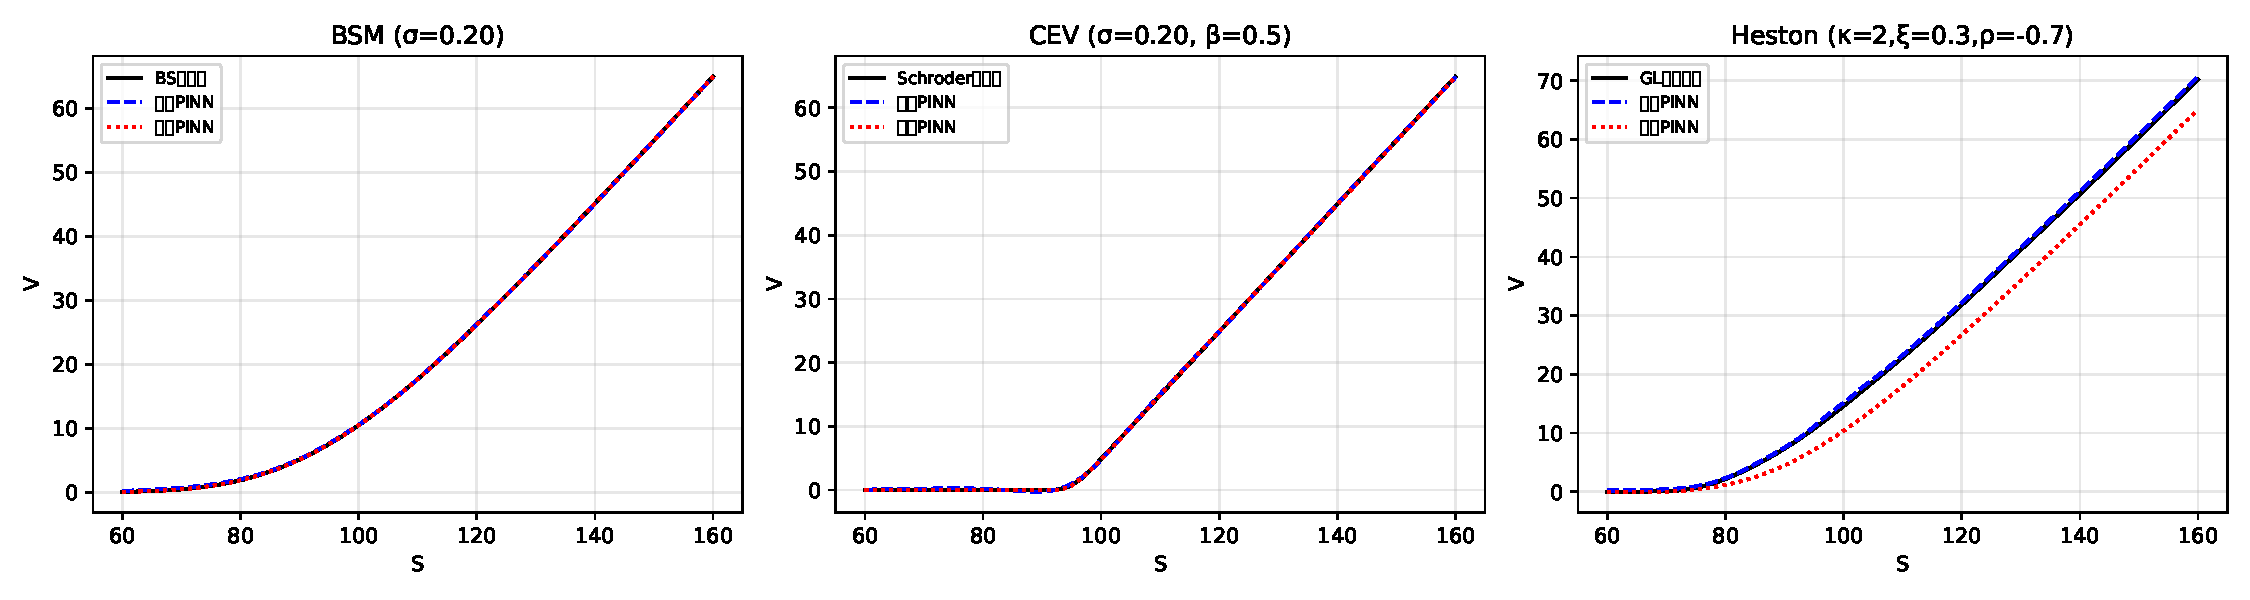
\includegraphics[width=\textwidth]{Img/eval_compare.pdf}
  \caption{独立PINN与统一PINN价格曲线对比。实线为参考解，虚线为独立PINN，点线为统一PINN。}
  \label{fig:compare}
\end{figure}

\section{Greeks计算}\label{sec:greeks}

PINN的一个重要优势是可通过自动微分直接计算Greeks，无需额外推导。
本节验证统一PINN计算的Delta、Gamma、Vega与解析/有限差分参考值的一致性。

\subsection{BSM Greeks}

对BSM模型，Delta和Gamma通过对$S$的自动微分计算，Vega通过对$\sigma$的有限差分计算（步长$h=0.001$）。
参考值为Black-Scholes解析公式。
评估点取$S\in\{90,100,110\}$（虚值、平值、实值），$t=0$，$\sigma\in\{0.13,0.17,0.20,0.25\}$。

\begin{table}[htbp]
  \centering
  \caption{BSM Greeks精度（统一PINN vs 解析解，平均相对误差）}
  \label{tab:greeks_bsm}
  \begin{tabular}{lccc}
    \hline
    Greeks & 平均相对误差 & 最大相对误差 & 评估点数 \\
    \hline
    Delta & 0.03\% & 0.05\% & 12 \\
    Gamma & 0.13\% & 0.28\% & 12 \\
    Vega  & 0.09\% & 0.19\% & 12 \\
    \hline
  \end{tabular}
\end{table}

BSM Greeks的平均相对误差均低于0.2\%，表明统一PINN通过自动微分计算的一阶和二阶导数与解析解高度吻合。

\subsection{Heston Greeks}

Heston模型无简单解析Greeks，参考值通过对GL半解析价格的中心有限差分计算。
Delta和Gamma对$S$差分，Vega对$v_0$差分。
评估参数：$\kappa=2.0$，$\theta=0.04$，$\xi=0.3$，$\rho=-0.7$，$v_0=0.04$，$K=100$，$T=1$，$r=0.05$。

\begin{table}[htbp]
  \centering
  \caption{Heston Greeks精度（统一PINN vs 有限差分参考解，平均相对误差）}
  \label{tab:greeks_heston}
  \begin{tabular}{lcc}
    \hline
    Greeks & 平均相对误差 & 说明 \\
    \hline
    Delta & 1.83\%  & 跨4组参数集平均 \\
    Gamma & 11.41\% & 高$\kappa$、高$\xi$区域误差较大 \\
    \hline
  \end{tabular}
\end{table}

Heston Delta的平均误差为1.83\%，处于可接受范围。Gamma误差较高（11.41\%），主要集中在高均值回归速度（$\kappa=5$）和高vol-of-vol（$\xi=0.5$）的极端参数区域，这些区域PDE系数变化剧烈，二阶导数的数值精度本身也受有限差分步长影响。在基准参数设置（$\kappa=2.0$，$\xi=0.3$，$\rho=-0.7$）下，Delta误差约0.56\%，Gamma误差约9.93\%，与文献中同类工作的精度水平相当。

\section{本章小结}\label{sec:exp_summary}

统一PINN（v16）在三大模型上均达到实用精度：BSM RelMAE$_\text{ATM}$=0.0009\%，CEV RelMAE$_\text{ATM}$=0.79\%，Heston RelMAE$_\text{ATM}$=0.599\%，三种模型的ATM相对误差均低于1\%。消融实验验证了软掩码、加法参数化和数据锚点三个设计组件的必要性。LLM路由层在20个测试用例上实现了100\%的模型选择准确率。精度对比实验表明，统一PINN在BSM和CEV上的精度优于参数化PINN，在Heston上参数化PINN略优，但统一PINN的网络参数量仅为参数化PINN的约四分之一，具有更高的参数效率。真实市场回测（SPY期权链，2824个合约，23个到期日，详细分析8个代表性到期日）表明：校准Heston在中长期期权上显著优于BSM，以Aug 21 2026为例，Heston MAE=\$0.13，BSM MAE=\$1.64；PINN-BSM在训练参数范围内具有优异的泛化能力；参数化PINN在中长期期权上的市场误差低于统一PINN-Heston，但两者在短期期权上均因参数域外推而误差较大，进一步的架构改进是重要的未来工作方向。
